
\section{Discussion}
The pattern documented in our analysis, from the 1987 crash to the persistent chicken problem across various debt securities, raises a fundamental question: why do market participants repeatedly fall into these traps?

The model that we started with suggests that individuals make probability calculations when they make decisions. Researchers have long pointed out, however, that individuals fail at even the most straightforward probabilistic calculations. Even colloquially, “the expected” often means “what comes to mind” rather than an actual calculation. This is not to suggest that people do not use models, such as the Black-Scholes-Merton model, or the copula models widely in use for the CDX contracts. Rather, they neither take these models seriously as true pictures of the world, not subjecting them to scrutiny that that would entail, nor do they form any conscious model, but rather make decisions based on what comes to mind. 

In the study of economics, we often seek to measure and to model this uncertainty, and the first step is typically a simplification. When we create a random variable, we are replacing a multi-, potentially infinite-dimensional object with something that has a fixed number of dimensions. Moreover, the idea of “expectation” (calculated as $E[X]$) has a strange consequence that the expected never happens: if you paid \$1 to earn \$2 if a coin were heads and \$0 if tails, you expect to earn \$1 on net from this gamble, yet that outcome can never occur. 

Perhaps we need a different way of thinking about finance and the unexpected. Recent research turns to evidence on memory to understand expectations. Our memories, and thus our thoughts and beliefs, are driven by: recency, similarity, and temporal contiguity.

Economists have long noted the strong pull of recent events on expectations. Recall that one of the questions that we are uncertain about was the return on the stock market (from Section 1). Several long-running surveys capture beliefs about this question. The Gallup survey asks respondents if they are very optimistic, optimistic, neutral, pessimistic, or very pessimistic. Campbell Harvey and co-authors surveyed CFOs about their expectations of stock returns over the next 12 months. These and more surveys were reviewed in a paper by \citet{greenwood2014expectations}.


\autoref{fig:fig16} \citep{greenwood2014expectations} shows the percentage of investors who are very optimistic or optimistic minus the percentage of investors who are pessimistic or very pessimistic, compared to stock returns from 12 months prior. The difference in this measure is well explained ($r^2 = 61 \%$ for Gallup) by returns from 12 months prior. Needless to say, this is not a good model for stock market returns. If anything, stock returns in aggregate exhibit negative autocorrelation over the relevant horizons. Recent events strongly influence the survey responses of these individuals. 

\begin{figure}[h]
    \centering
    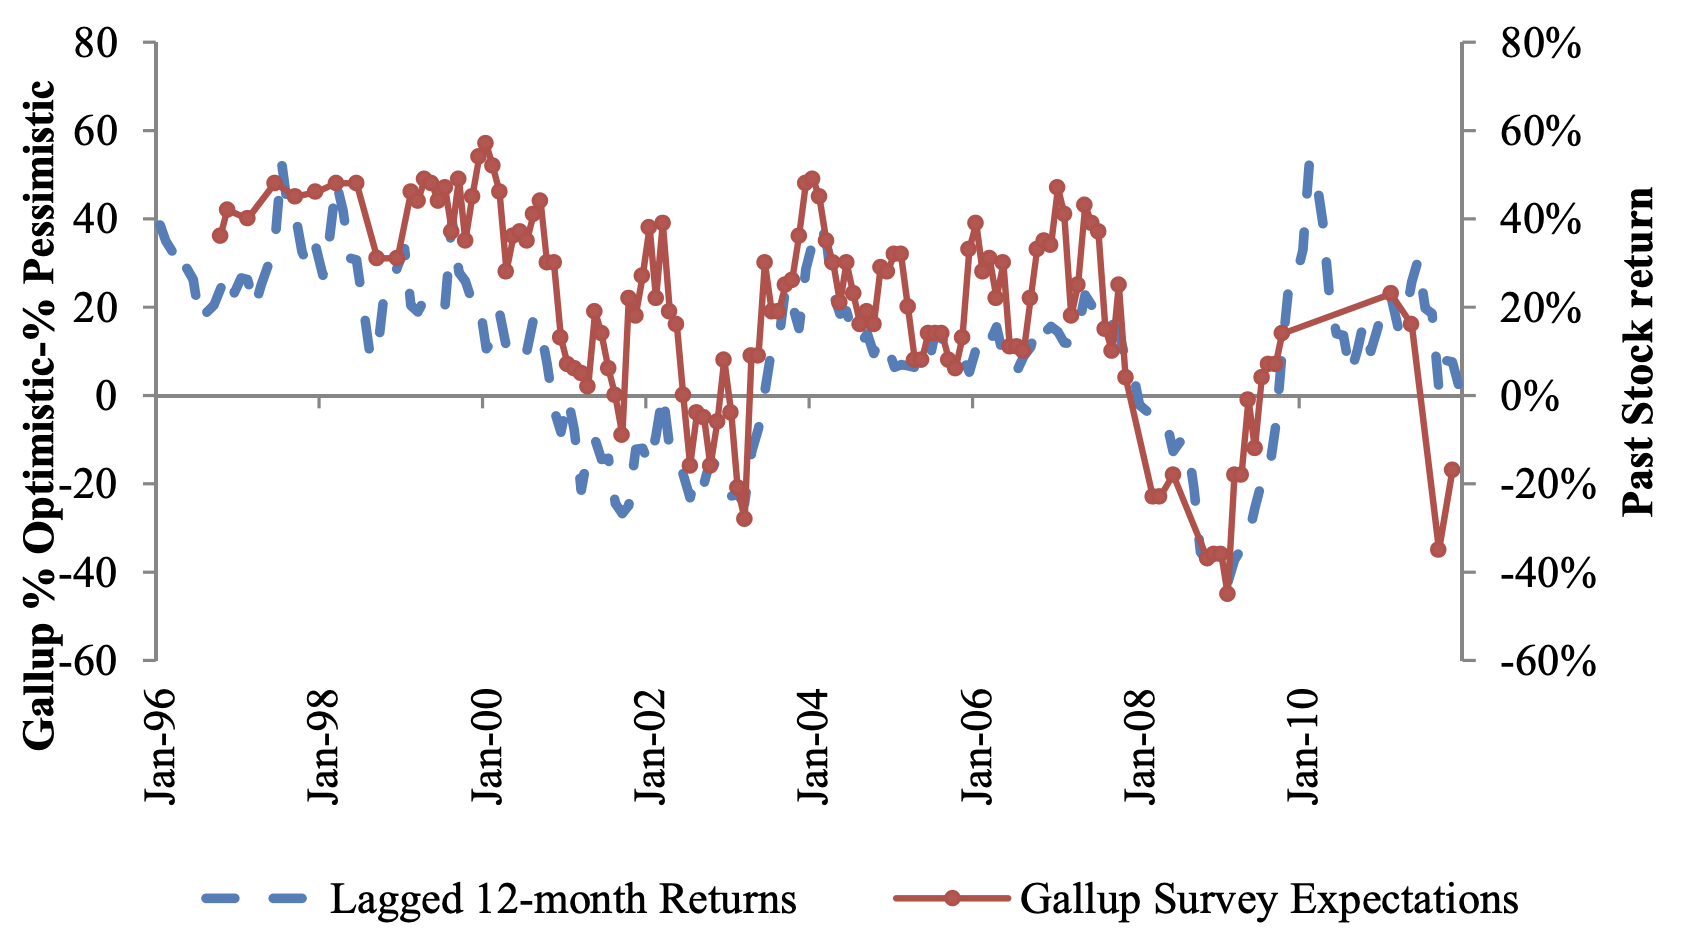
\includegraphics[width=0.75\textwidth]{fig16.png}
    \caption{Gallup survey responses compared to shifted stock returns \citep{greenwood2014expectations}}
    \label{fig:fig16}
\end{figure}

Recall the problem faced by the chicken. Even with no recency bias, it is difficult to infer the underlying distribution of events when faced only with data and with an incorrect model. A little imagination might have helped the chicken. However, if our beliefs are pulled toward recent events, that will make it even more difficult to have this imagination.

There are some important caveats to recency, as recent experiences are a subset of experience. Researchers have also shown that experience matters, both past and present. One 2009 study showed that experience moderates the effects of recency \citep{greenwood2014expectations}. The authors studied asset managers' holdings during the dot-com bubble by regressing change in holdings in technology stocks on age in each quarter. \autoref{fig:fig17} \citep{greenwood2009inexperienced} shows the coefficients plotted against the returns in that quarter. They found that the dependence on past returns decreased, the older the asset manager. That is, younger managers tended to chase trends whereas older ones were contrarians. The higher the returns, the more likely it is younger managers investing and older managers dis-investing.

\begin{figure}[h]
    \centering
    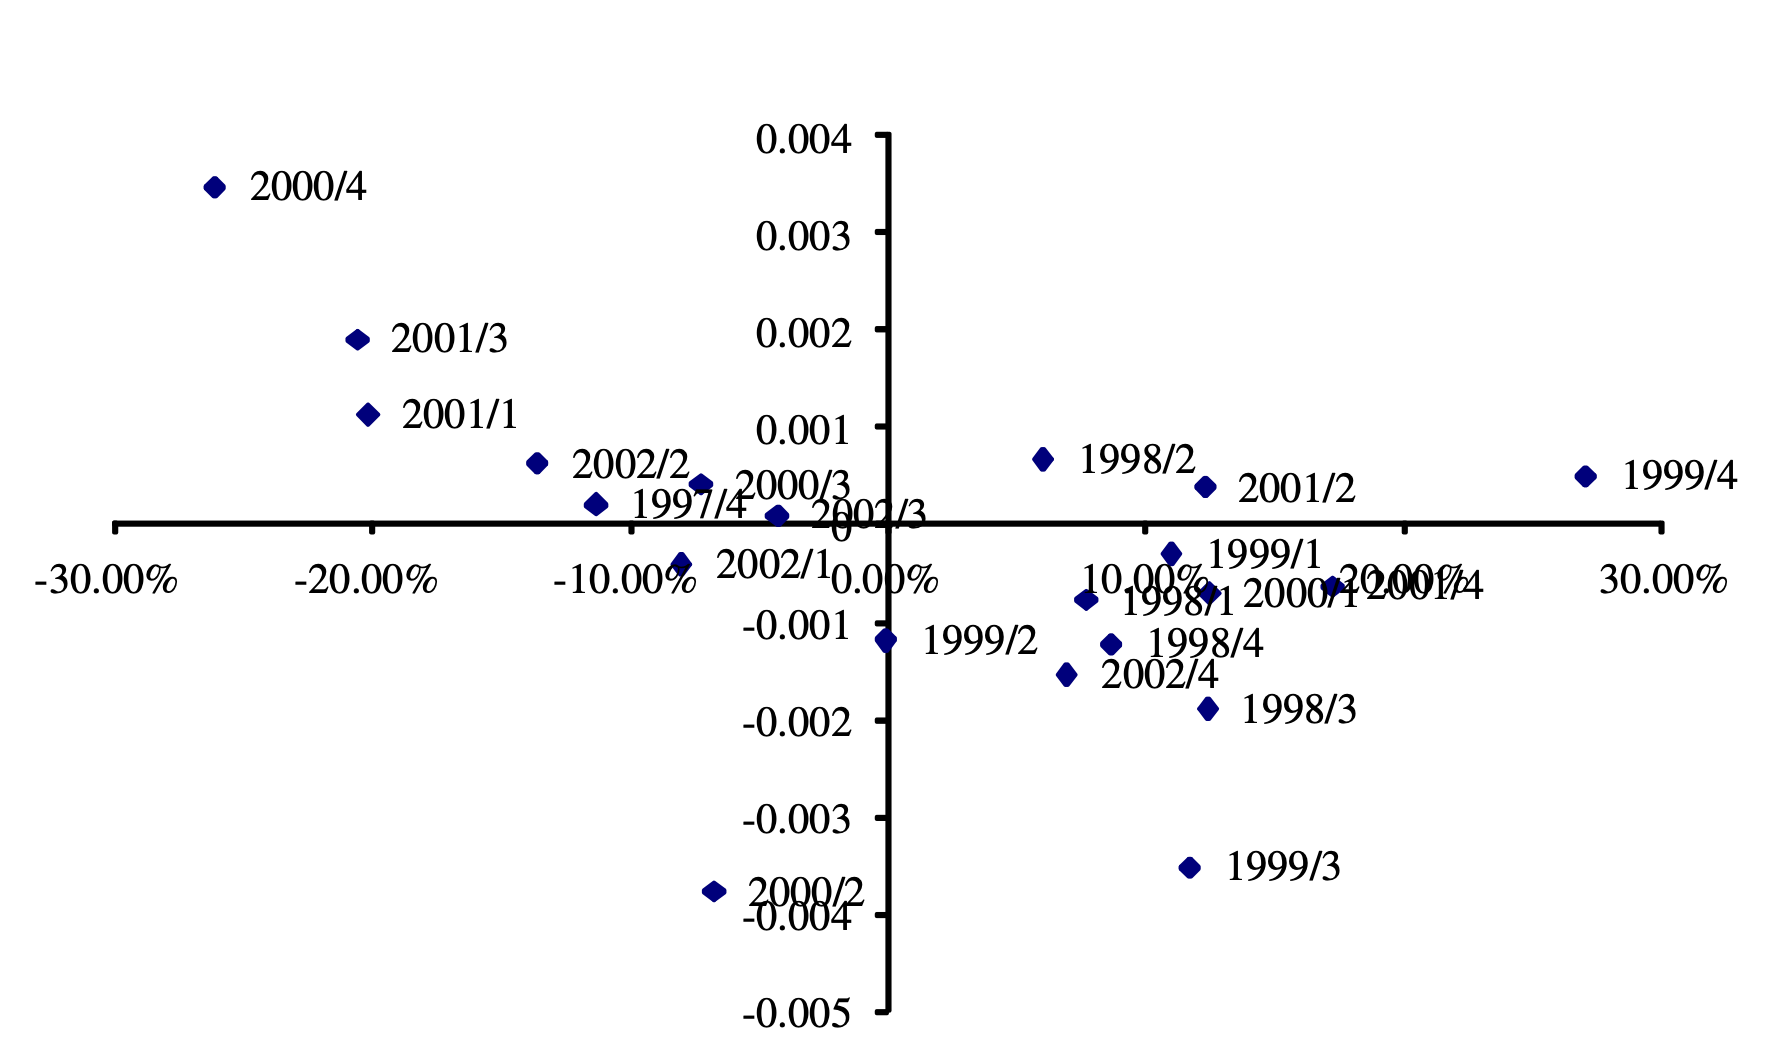
\includegraphics[width=0.65\textwidth]{fig17.png}
    \caption{Regressing age with change in managers' holdings \citep{greenwood2009inexperienced}}
    \label{fig:fig17}
\end{figure}

This study has the remarkable conclusion that early life experience in the stock market is apparently never forgotten. The importance of experience is a link between financial decisions, and the relevance of free recall in the laboratory. Because if experience matters, then memory matters. And free recall is the study of memory.

When an event is recalled, memory is biased toward other events that occurred close in time. This clustering effect is called temporal contiguity \citep{howard2002distributed}. Temporal contiguity is thought to arise because recalling an item reinstates the mental context from when it was first learned, and that reinstated context makes nearby memories easier to access.

According to context-maintenance models of memory, individuals’ thoughts and beliefs are governed by an internal context. Information from the environment retrieves a context that depends on the features filtered through past memories: the individual retrieves past contexts in which similar features were experienced. Retrieved context averages with past context to form current context. Current context determines what comes to mind. This framework helps explain why we sometimes struggle to recall specific details while also accounting for the fact that memories are rarely lost entirely.

Moreover, mental context has broader implications for decision-making. Associations formed in one context can lead to very different responses than those formed in another. As underlying mental associations evolve, the decisions that stem from them can change as well. Deciding how to invest and how much are some of the most important financial decisions an investor can make. Recent literature has turned to the role of lifetime experience in shaping these choices. \citet{malmendier2021memory} show that lifetime stock market performance is a major determinant of whether an individual chooses to participate at all (\autoref{fig:fig18}). People with better lifetime market experiences (e.g., those in the 90th percentile of lifetime market performance) are 10 percentage-points more likely to invest than those with worse experiences (e.g., those in 10th percentile), in a sample where the average participation rate is 34\%. The magnitude of these experience effects is comparable to that of other well‑established determinants, including income and education.

\begin{figure}[h]
    \centering
    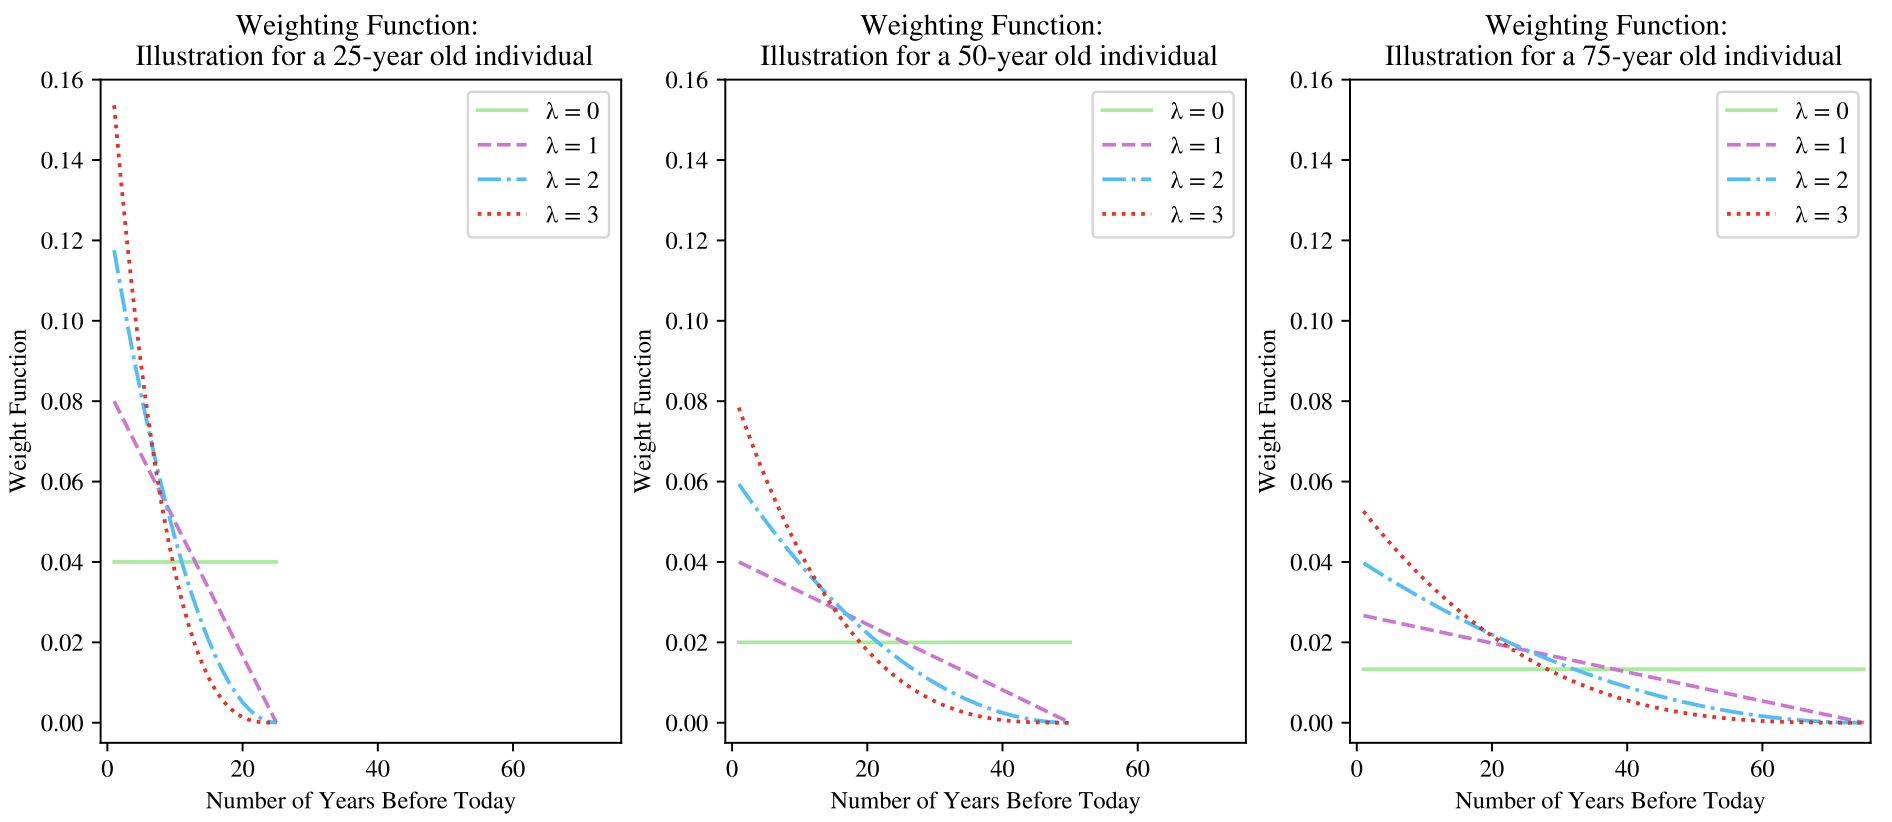
\includegraphics[width=0.75\textwidth]{fig18.png}
    \caption{Weight of past experiences changes with age \citep{malmendier2021memory}}
    \label{fig:fig18}
\end{figure}

Multiple findings relevant to financial data reflect these results. \citet{guiso2018time} examined risk aversion in an experiment with the same set of participants before and after the 2008 crisis. The participants, who were professional traders, required twice the premium to accept a bet following the crisis as before. The people were the same, the bets were the same, but the associations had changed. The same study also performed an experiment in which undergraduates watched a scene from a horror movie: those who watched the scene required a 50\% greater premium to invest than those that did not. 

Another study \citep{cohn2015evidence} experimentally manipulated context by presenting study participants, who were professional traders, with scenarios involving a normal trading day versus a stock market crash. The traders were then presented with risky bets with various degrees of return. Those with the market crash context required a higher premium to accept the risky bet. Both the horror movie and crash simulations represented context manipulations that affected behavior.  
 
Ultimately understanding the unexpected in finance means grappling with the unexpected in human decision-making. We believe that research in memory offers one path forward.
